\documentclass[11pt]{article}

% -------- PAQUETES --------
\usepackage[spanish]{babel}
\usepackage[utf8]{inputenc}
\usepackage[T1]{fontenc}
\usepackage{times}
\usepackage{setspace}
\usepackage[left=2.5cm, right=2.5cm, top=2.5cm, bottom=2.5cm]{geometry}
\usepackage{ragged2e}
\usepackage{graphicx}
\usepackage{subcaption}
\usepackage{fancyhdr}
\usepackage{hyperref}
\usepackage{tocloft}

% -------- CONFIGURACIONES --------
\setstretch{2}
\setlength{\parskip}{0pt}
\setlength{\parindent}{5ex}
\justifying
\pagestyle{fancy}
\fancyhf{}
\rhead{
\includegraphics[width=3cm]{img/logoTecAzuay.png}}
\renewcommand{\headrulewidth}{0pt}
\cfoot{\thepage}
%\renewcommand{\cftsecleader}{\cftdotfill{\cftdotsep}}
%\renewcommand{\cftsubsecleader}{\cftdotfill{\cftdotsep}}

% -------- INFORME --------
\begin{document}

    \thispagestyle{empty}
    \begin{center}

        \begin{figure}
            \centering         
            
\includegraphics[width=0.5\textwidth]{img/logoTecAzuay.png} 
        \end{figure} 

        \textbf{
            TECNOLOGÍA SUPERIOR EN MECATRÓNICA \\ 
            PROYECTO DE TUTORÍAS INTEGRADAS 
        }
        
        \textbf{\\ TEMA: \\} Generación de energía eléctrica a través de microgeneradores hidroeléctricos y una estación de carga \\ Parte 1: Análisis de viabilidad \\\
       
        \textbf{ESTUDIANTES:\\} Eduardo Mendieta - Christian Sanchez 

        \textbf{TUTORES ACADÉMICOS: \\} Ing. Pedro Martínez - Ing. Daniela Sarango

        \textbf{TUTOR EMPRESARIAL: \\} Ing. Juan Pablo Arichávala

        \textbf{CICLO: \\} Primer ciclo - Tercer ciclo

        \textbf{CIUDAD: \\} Cuenca
        
        \textbf{PERIÓDO ACADÉMICO: \\} Octubre 2023 - Febrero 2024

    \end{center}



    \tableofcontents \newpage


    % === 1.
    \section{Tema del proyecto}
    Generación de energía eléctrica a través de microgeneradores hidroeléctricos y una
    estación de carga - Parte 1: Análisis de viabilidad.

    % === 2.
    \section{Localización}

    \textbf{Sede y ámbito de estudio:} 
    El presente estudio se realiza en las instalaciones de Continental Tire Andina S.A., ubicadas
    en la ciudad de Cuenca, Azuay. Específicamente, se lleva a cabo en la torre de enfriamiento
    de agua destinada a las maquinarias Triplex, Roller Head y Mixer 4.

    \textbf{Dirección:} Panamericana N KM-2.8, Calle S/N, Cuenca, Azuay. 

    \textbf{Descripción de Continental Tire Andina S.A.:}
    Continental Tire Andina S.A. es una empresa integrante del grupo Continental, dedicada a la
    fabricación y comercialización de neumáticos en América Latina. Enfocada en satisfacer las
    necesidades del mercado sudamericano, ofrece una amplia gama de neumáticos para
    automóviles, camiones y maquinaria pesada, así como servicios relacionados con los
    mismos.

    \textbf{Misión:}
    Su misión es crear un entorno laboral que fomente el crecimiento y desarrollo del personal.
    Buscando mejorar la satisfacción del cliente mediante la entrega de productos de calidad,
    rápida atención y optimización de costos. Se comprometen a adoptar una cultura de mejora
    continua para asegurar un crecimiento rentable y sostenible.

    \textbf{Visión:}
    Se proyectan como el distribuidor de llantas más confiable de la región Andina, ofreciendo
    productos y servicios de primera calidad. Se diferencian por su profundo conocimiento y
    entendimiento de las necesidades del cliente, lo que les permite brindar soluciones
    personalizadas y efectivas.

    % === 3.
    \section{Análisis de la situación actual}
    Actualmente, se emplea un sistema de circulación de agua en ciclos para el enfriamiento de
    las maquinarias Triplex y Roller Head, así como para el funcionamiento de las unidades de
    control de temperatura (TCU) asociadas con la maquinaria Roller Head, encargadas de
    calentar el agua utilizada en la cabeza y los tornillos. Además, en el caso de la maquinaria
    Mixer 4, el agua se utiliza tanto para los procesos de calentamiento mediante TCUs como
    para el enfriamiento del motor.
    
    El agua utilizada en estos procesos anteriormente descritos retorna a una torre de
    enfriamiento ubicada en las instalaciones exteriores, donde se enfría antes de ser
    bombeada nuevamente mediante motores con una presión fluctuante entre 50 y 60 psi a
    través de una tubería con un diámetro aproximado de 22.2816 cm, para reiniciar el ciclo de
    enfriamiento y calentamiento en las maquinarias mencionadas.

    % === 4.
    \section{Antecedentes}
    En el marco del plan de estudios de la carrera de Mecatrónica en el Instituto Superior
    Universitario Tecnológico del Azuay, se destaca la necesidad de desarrollar proyectos
    empresariales como parte integral de la formación académica. Una propuesta relevante
    dentro de este contexto es la creación de un proyecto enfocado en la generación de energía
    eléctrica mediante microgeneradores disponibles en el mercado, aprovechando la alta
    presión del agua en movimiento. El objetivo principal radica en acumular esta energía para
    su posterior aplicación en diversos ámbitos, lo cual representa un desafío interesante en
    términos de innovación tecnológica y sostenibilidad.

    Por otro lado, en Continental Tire Andina S.A., se ha identificado una oportunidad para
    aprovechar el flujo de agua a alta presión utilizado en los procesos de la empresa para
    generar energía eléctrica. Esta propuesta busca instalar múltiples generadores a lo largo de
    las tuberías, aprovechando la energía cinética del agua en circulación. El almacenamiento
    de la energía resultante se plantea como un componente fundamental, destinado a
    establecer una central eléctrica o estación de carga capaz de satisfacer las demandas
    energéticas de dispositivos con diferentes requisitos de voltaje y amperaje. Este proyecto no
    solo busca optimizar los recursos disponibles, sino también implementar un control
    específico mediante software personalizado para garantizar una gestión eficiente de la
    energía generada.

    % === 5.
    \section{Justificación de la propuesta}
        \begin{itemize}
            \item La presencia constante de un sistema de circulación de agua en funcionamiento
            continuo, operativo las 24 horas del día, los 7 días de la semana, junto con un flujo
            bajo alta presión de 50 a 60 psi a través de una tubería de diámetro considerable de
            aproximadamente 22.2816 cm, ofrece una oportunidad excepcional para aprovechar
            la energía cinética del agua. Este recurso hidrocinético representa una fuente
            inagotable de energía que, mediante micro generadores hidroeléctricos, puede
            convertirse eficientemente en electricidad.

            \item La energía generada no sólo satisfará las necesidades energéticas de la empresa,
            sino que también proporcionará un valioso respaldo energético, garantizando la
            continuidad de las operaciones en caso de cortes de suministro eléctrico externo y
            generando beneficios económicos a largo plazo al reducir la dependencia de la red
            eléctrica convencional.

            \item La implementación de un sistema de generación eléctrica localizado y basado en
            fuentes renovables, específicamente la energía hidrocinética, demuestra el
            compromiso de la empresa con la sostenibilidad y la responsabilidad ambiental. Al
            optar por una fuente de energía limpia y renovable, se contribuye a la mitigación del
            cambio climático y se avanza en los objetivos de sostenibilidad corporativa,
            estableciendo un precedente positivo para el sector industrial en general.

        \end{itemize}    
   
    % === 6.
    \section{Población beneficiaria}
    Los beneficiarios del presente proyecto se encuentran divididos en dos categorías
    principales. En primer lugar, destaca la empresa Continental Tire Andina S.A., la cual se
    verá favorecida por la implementación de esta iniciativa, la cual tiene como objetivo principal
    proporcionar una fuente adicional de energía eléctrica para sus instalaciones. Por otro lado,
    se encuentran los estudiantes responsables del desarrollo de este proyecto, quienes
    obtienen la oportunidad de poner en práctica sus conocimientos adquiridos y de
    involucrarse en un proyecto con aplicaciones tangibles en el contexto de la vida real.
        
    % === 7.
    \section{Objetivos}

        \subsection{Objetivo general}
        Elaborar un análisis exhaustivo de viabilidad destinado a evaluar la implementación de un
        sistema de generación de energía eléctrica utilizando micro generadores hidroeléctricos,
        junto con una estación de carga, específicamente para el área de Planta Común de la
        empresa Continental Tire Andina S.A.
        
        \subsection{Objetivos específicos}
            \begin{itemize}
                \item Realizar una investigación exhaustiva sobre los fundamentos asociados a la
                generación de energía hidroeléctrica mediante micro generadores, así como las
                estrategias óptimas para el almacenamiento de energía y la gestión integral del
                sistema a desarrollar, con el fin de establecer un marco conceptual preciso para el
                proyecto.

                \item Analizar la viabilidad de emplear la energía producida con el propósito de abastecer
                las baterías de los montacargas tipo TCM y Prime Mover pertenecientes a la
                infraestructura de la empresa, como una alternativa para la distribución eficiente de
                la energía eléctrica generada por el sistema propuesto.

                \item Presentar un análisis exhaustivo de los aspectos positivos y negativos relacionados
                con la implementación de un sistema de generación de energía eléctrica mediante
                micro generadores y estaciones de carga, con el fin de evaluar de manera integral la
                viabilidad del proyecto.
                
            \end{itemize}
      
    % === 8.
    \section{Marco teórico}
            \subsection{Fundamentos de la generación de energía hidroeléctrica mediante micro
                        generadores}
            La generación de energía hidroeléctrica mediante microgeneradores aprovecha la energía
            cinética del agua en movimiento para convertirla en energía eléctrica. Este enfoque ofrece
            una solución sostenible y limpia para la producción de electricidad en lugares donde hay
            corrientes de agua disponibles, como salidas de torres de enfriamiento. 

            
            \subsubsection{Principios Básicos}

            \textbf{Principio de conversión de energía:} La generación de energía hidroeléctrica se basa en el
            principio de la conversión de energía, donde la energía cinética del agua en movimiento se
            transforma en energía eléctrica utilizable.

            \textbf{Microgeneradores: } Los microgeneradores hidroeléctricos son dispositivos compactos
            diseñados para generar electricidad en pequeña escala. Utilizan una variedad de
            tecnologías, como turbinas de flujo, generadores de presión o generadores de flujo
            transversal, para aprovechar la energía del agua y producir energía eléctrica.
            
            
            \subsubsection{Componentes principales}

            \textbf{Turbina o rotor:} El componente principal de un microgenerador hidroeléctrico es la turbina o
            el rotor, que convierte la energía cinética del agua en movimiento en energía mecánica.
            
            \textbf{Generador eléctrico:} La energía mecánica generada por la turbina se transfiere a un
            generador eléctrico, que convierte esta energía mecánica en energía eléctrica mediante el
            principio de inducción electromagnética.

            \textbf{Sistema de control y regulación:} Los microgeneradores hidroeléctricos suelen estar
            equipados con sistemas de control y regulación para optimizar su rendimiento y garantizar
            una operación segura y eficiente.

            \subsubsection{ Factores que afectan la generación de energía}

            \textbf{Caudal de ggua:} El caudal de agua, es decir, la cantidad de agua que pasa por el
            microgenerador en un período de tiempo dado, es un factor crucial que afecta la cantidad de
            energía que se puede generar.

            \textbf{Altura de caída o presión:} La altura de caída del agua o la presión del agua disponible
            determinan la energía potencial del agua, que es crucial para la generación de energía
            hidroeléctrica.

            \textbf{Eficiencia del sistema:} La eficiencia del sistema, que incluye la eficiencia de la turbina, el
            generador y otros componentes, influye en la cantidad de energía eléctrica que se puede
            producir a partir de la energía hidroeléctrica disponible.

            
            \subsubsection{Ventajas de la Generación de Energía Hidroeléctrica}

            \textbf{Fuente renovable y sostenible:} La energía hidroeléctrica es una fuente de energía
            renovable y sostenible, ya que utiliza el ciclo natural del agua y no produce emisiones de
            gases de efecto invernadero.

            \textbf{Bajo impacto ambiental:} En comparación con otras formas de generación de energía, como
            la quema de combustibles fósiles, la generación de energía hidroeléctrica tiene un impacto
            ambiental relativamente bajo, especialmente en proyectos a pequeña escala.
            
            \textbf{Localización flexible:} Los microgeneradores hidroeléctricos pueden instalarse en una
            variedad de ubicaciones, incluidos arroyos, ríos, canales o salidas de torres de enfriamiento,
            lo que permite una mayor flexibilidad en su implementación.
            
            En resumen, la generación de energía hidroeléctrica mediante microgeneradores ofrece una
            forma eficiente y sostenible de producir electricidad, aprovechando el potencial energético
            del agua en movimiento en diversas ubicaciones.


            \subsection{Sistemas de almacenamiento de energía eléctrica}
            Los sistemas de almacenamiento de energía eléctrica son tecnologías diseñadas para
            acumular energía en forma de electricidad para su uso posterior. Estos sistemas
            desempeñan un papel crucial en la gestión eficiente y flexible de la energía, permitiendo la
            integración de fuentes de energía intermitentes, como la solar y la eólica, en las redes
            eléctricas.

            Los sistemas de almacenamiento de energía eléctrica pueden variar en tamaño y
            capacidad, desde baterías pequeñas utilizadas en aplicaciones residenciales hasta grandes
            instalaciones a escala de red que pueden almacenar energía a nivel industrial. Además,
            estas tecnologías pueden aprovechar una variedad de métodos de almacenamiento, como
            el almacenamiento químico en baterías, el almacenamiento mecánico en forma de
            almacenamiento por bombeo de agua o volantes de inercia, y el almacenamiento térmico.
            
            Al permitir la captura y liberación de energía de manera eficiente, los sistemas de
            almacenamiento de energía eléctrica contribuyen a mejorar la estabilidad de las redes
            eléctricas, reducir los picos de demanda, optimizar la utilización de fuentes renovables y
            proporcionar respaldo durante cortes de energía. En última instancia, estos sistemas juegan
            un papel fundamental en la transición hacia un sistema energético más sostenible y
            resiliente. 

            \subsubsection{Características clave de los sistemas de almacenamiento de energía eléctrica}
            

            Los sistemas de almacenamiento de energía eléctrica son componentes fundamentales en
            la infraestructura energética moderna, permitiendo la integración efectiva de fuentes de
            energía intermitentes y la gestión eficiente de la demanda de energía. En la evaluación y
            selección de estos sistemas, es crucial considerar una serie de características clave que
            influyen en su rendimiento, viabilidad y efectividad. A continuación, se describen las
            principales características a tener en cuenta:

            \begin{enumerate}
                \item \textbf{ Capacidad de almacenamiento:} La capacidad de almacenamiento de un sistema de energía eléctrica se refiere a la cantidad
                máxima de energía que puede ser almacenada y posteriormente liberada cuando sea
                necesario. Esta capacidad se mide comúnmente en kilovatios-hora (kWh) o
                megavatios-hora (MWh), y es un factor determinante en la capacidad del sistema para
                satisfacer la demanda de energía durante períodos de alta demanda o baja disponibilidad
                de energía.

                \item \textbf{Eficiencia energética:} La eficiencia energética de un sistema de almacenamiento se refiere a la relación entre la
                energía almacenada y la energía consumida durante el proceso de carga y descarga. Una
                alta eficiencia energética es deseable ya que minimiza las pérdidas de energía durante el
                ciclo de almacenamiento y recuperación, lo que a su vez mejora la rentabilidad y la
                sostenibilidad del sistema.

                \item \textbf{Tiempo de respuesta:} El tiempo de respuesta de un sistema de almacenamiento de energía eléctrica indica la
                rapidez con la que puede cambiar entre los modos de carga y descarga de energía. Un
                tiempo de respuesta rápido es crucial para garantizar la disponibilidad inmediata de energía
                cuando sea necesario, lo que es especialmente importante en aplicaciones críticas donde
                se requiere una respuesta rápida a cambios en la demanda de energía.

                \item \textbf{Vida útil:} La vida útil de un sistema de almacenamiento de energía eléctrica se refiere al período de
                tiempo durante el cual el sistema puede operar de manera efectiva y confiable antes de
                necesitar ser reemplazado o requiere mantenimiento significativo. Una vida útil más larga es
                deseable ya que reduce los costos de mantenimiento y reemplazo a lo largo del tiempo, lo
                que mejora la rentabilidad y la viabilidad del sistema.

                \item \textbf{Costo:} El costo total de propiedad de un sistema de almacenamiento de energía eléctrica incluye
                tanto los costos iniciales de adquisición e instalación como los costos operativos y de
                mantenimiento a lo largo de la vida útil del sistema. Es fundamental evaluar los costos en
                relación con otros beneficios y consideraciones para determinar la viabilidad económica del
                sistema.

                \item \textbf{Modularidad y escalabilidad:} La modularidad y escalabilidad de un sistema de almacenamiento se refiere a su capacidad
                para adaptarse y crecer según sea necesario para satisfacer los cambios en la demanda de
                energía. Esta capacidad proporciona flexibilidad operativa y permite una optimización
                continua del sistema a medida que evolucionan las necesidades energéticas.
            \end{enumerate}

            

            \ \subsubsection{Consideraciones para la implementación de sistemas de almacenamiento de energía
                             eléctrica} 
            
                             La implementación efectiva de sistemas de almacenamiento de energía eléctrica requiere
                             una cuidadosa consideración de una serie de factores clave que influyen en su rendimiento,
                             viabilidad y efectividad en el contexto específico de aplicación. A continuación, se describen
                             algunas consideraciones importantes que deben tenerse en cuenta al planificar e
                             implementar estos sistemas:

            \begin{enumerate}
                \item \textbf{Análisis de la demanda energética:} Antes de seleccionar y dimensionar un sistema de almacenamiento de energía eléctrica, es
                fundamental realizar un análisis exhaustivo de la demanda energética del sitio o la
                aplicación específica. Esto incluye evaluar los patrones de consumo de energía, identificar
                picos de demanda y determinar los requisitos de potencia y energía necesarios para
                satisfacer las necesidades del usuario.

                \item \textbf{Integración con fuentes de energía renovable:} Para maximizar el valor y la efectividad de un sistema de almacenamiento de energía, es
                importante considerar su integración con fuentes de energía renovable, como la solar, eólica
                o hidroeléctrica. Estas fuentes intermitentes pueden beneficiarse significativamente de la
                capacidad de almacenamiento para mitigar la variabilidad y la intermitencia de la generación
                de energía.

                \item \textbf{Selección del tipo de tecnología de almacenamiento:} Existen varias tecnologías de almacenamiento de energía eléctrica disponibles, cada una
                con sus propias características, ventajas y limitaciones. Es crucial evaluar cuidadosamente
                las opciones disponibles y seleccionar la tecnología más adecuada en función de los
                requisitos de rendimiento, costos, vida útil, eficiencia y otras consideraciones específicas del
                proyecto.

                \item \textbf{Evaluación de viabilidad económica:} La viabilidad económica de un sistema de almacenamiento de energía eléctrica es un factor
                determinante en su implementación exitosa. Se deben realizar análisis detallados de costos
                y beneficios para evaluar el retorno de la inversión, considerando tanto los costos iniciales
                de adquisición e instalación como los costos operativos y de mantenimiento a lo largo de la
                vida útil del sistema.

                \item \textbf{Planificación del ciclo de vida y mntenimiento:} La planificación del ciclo de vida y el mantenimiento adecuado son fundamentales para
                garantizar el rendimiento óptimo y la confiabilidad a largo plazo del sistema de
                almacenamiento de energía eléctrica. Se deben establecer programas de mantenimiento
                preventivo y predictivo, así como planes de gestión de riesgos y contingencias para abordar
                posibles fallas o problemas operativos. 

            \end{enumerate}
            

            \subsection{Control y monitoreo de sistemas de generación de energía eléctrica}
            El control y monitoreo efectivos son fundamentales para garantizar el rendimiento óptimo y
            la fiabilidad de los sistemas de generación de energía eléctrica basados en
            microgeneradores hidroeléctricos. Estos sistemas operan en entornos variables y pueden
            estar sujetos a fluctuaciones en el caudal del agua, cambios climáticos y otros factores
            externos. Por lo tanto, un sistema de control robusto y un monitoreo preciso son esenciales
            para maximizar la eficiencia de la generación de energía y garantizar su funcionamiento
            continuo.

            \subsubsection{Componentes recomendados para un sistema de control y monitoreo}

            \textbf{Sensores de caudal y presión:} Los sensores de caudal y presión proporcionan mediciones
            precisas del flujo de agua y las condiciones hidráulicas dentro de la tubería. Estos sensores
            pueden ser ultrasónicos, electromagnéticos o basados en tecnología de presión, y se
            utilizan para monitorear el rendimiento de la turbina y detectar posibles obstrucciones o
            problemas de flujo.

            \textbf{Controladores programables (PLC):} Los PLC son dispositivos electrónicos programables
            que se utilizan para controlar y supervisar procesos automatizados. En el contexto de los
            sistemas de generación hidroeléctrica, los PLC se utilizan para implementar algoritmos de
            control, gestionar la comunicación con sensores y dispositivos, y ejecutar acciones de
            respuesta según las condiciones del sistema.

            \textbf{Software de análisis de datos:} Herramientas de análisis de datos como MATLAB, Python
            con bibliotecas como Pandas y NumPy, o herramientas específicas para el análisis de
            series temporales, permiten procesar grandes volúmenes de datos generados por el
            sistema de monitoreo. Estos programas facilitan la identificación de tendencias, la detección
            de anomalías y la optimización del rendimiento del sistema.


            \subsection{Tipos de micro generadores y su adecuación a características específicas de
            presión y caudal de agua.}
            Los microgeneradores hidroeléctricos pueden variar en diseño y tecnología, y su elección
            depende en gran medida de las características específicas del sitio, como la presión y el
            caudal de agua disponibles. A continuación se presentan algunos tipos comunes de
            microgeneradores y su adecuación a diferentes condiciones de operación:

            \begin{itemize}
                \item \textbf{Turbina de flujo} Las turbinas de flujo son dispositivos que aprovechan el flujo de agua para
                generar energía mecánica. Pueden ser de varios tipos, como turbinas de flujo axial, turbinas
                de flujo radial o turbinas de flujo mixto.
                
                \textbf{Adecuación:} Las turbinas de flujo son adecuadas para sitios con un caudal de agua
                moderado a alto y una presión relativamente baja. Son eficaces en sitios con un flujo
                constante y pueden adaptarse a diferentes niveles de caída vertical.
                
                \item  \textbf{Generador de presión}
                Los generadores de presión aprovechan la presión del agua en lugar del flujo
                para generar energía. Estos sistemas pueden utilizar una boquilla estrecha para aumentar
                la velocidad del agua y generar presión, que luego se convierte en energía mecánica y
                eléctrica.

                \textbf{Adecuación: }Los generadores de presión son ideales para sitios con una presión de agua
                alta pero un caudal moderado. Son eficientes en lugares donde la caída vertical es limitada
                pero la presión del agua es significativa, como las salidas de las torres de enfriamiento.
                
                \item \textbf{Generador de flujo transversal}
                Los generadores de flujo transversal son dispositivos que aprovechan el flujo
                de agua a través de una sección transversal para generar energía. Utilizan la fuerza del
                agua que pasa a través de la turbina para generar energía mecánica.
                
                \textbf{Adecuación:} Los generadores de flujo transversal son adecuados para sitios con un caudal
                de agua moderado y una presión relativamente baja. Son particularmente eficientes en
                lugares donde el flujo de agua es constante y la caída vertical es limitada.
                
                \item \textbf{Otros tipos específicos:}
                Además de los tipos mencionados, existen otros tipos específicos de
                microgeneradores hidroeléctricos, como los sistemas de tornillo Archimedes o los sistemas
                de vórtice, que pueden ser adecuados para condiciones particulares de presión y caudal de
                agua.

                \textbf{Adecuación:} Estos sistemas pueden ser adecuados para aplicaciones específicas donde las
                condiciones de presión y caudal de agua son únicas y requieren soluciones personalizadas.
            \end{itemize}

            
            \subsubsection{Selección del tipo de microgenerador}

            La selección del tipo de microgenerador más adecuado depende de una evaluación
            detallada de las características del sitio, incluyendo el caudal y la presión del agua
            disponibles, así como la variabilidad estacional y otros factores ambientales y operativos.
            

            \subsection{ Aplicación de la energía producida en la alimentación de las baterías de los
            montacargas tipo TCM y Prime Mover.}

            La energía generada a través de los microgeneradores hidroeléctricos se utilizará
            inicialmente para alimentar los cargadores de las baterías de 24V, que a su vez se
            encargarán de cargar las baterías de los montacargas tipo TCM y Prime Mover. Estos
            cargadores transforman la energía hidroeléctrica recibida en una salida de voltaje en
            corriente continua (DC) de 24V, que coincide con el voltaje de las baterías utilizadas en los
            montacargas.

            \textbf{Funcionamiento del proceso de carga:}
            Alimentación de los Cargadores: La energía eléctrica generada por los microgeneradores
            hidroeléctricos se suministra a los cargadores de baterías instalados en las instalaciones de
            carga de la empresa.

            \textbf{Transformación y regulación de la energía:} Los cargadores de baterías transforman y
            regulan la energía recibida para proporcionar una salida de voltaje de 24V en corriente
            continua (DC), que es compatible con las baterías de los montacargas.
            Conexión y Carga de las Baterías: Una vez que se alcanza la salida de voltaje deseada, las
            baterías de 24V de los montacargas se conectan a los cargadores y se inicia el proceso de
            carga. Las baterías reciben la energía necesaria para su recarga y mantenimiento.
            
            \textbf{Monitoreo y control: }Durante el proceso de carga, los cargadores de baterías supervisan y
            controlan varios parámetros, como la corriente de carga, el estado de carga de las baterías
            y la temperatura, para garantizar una carga segura y eficiente.
            Beneficios de la Alimentación de Cargadores y Carga de Baterías:
            
            \textbf{Optimización de la eficiencia energética: }Al utilizar energía hidroeléctrica para alimentar los
            cargadores de baterías, se logra una mayor eficiencia energética en comparación con los
            métodos convencionales de generación de energía.
           
           \textbf{Compatibilidad y fiabilidad:} La salida de voltaje de 24V proporcionada por los cargadores
            de baterías es compatible con las baterías de los montacargas tipo TCM y Prime Mover,
            asegurando un rendimiento óptimo y una carga confiable.

            \textbf{Cumplimiento ambiental:} Al adoptar prácticas sostenibles de generación de energía y
            transporte, la empresa demuestra su compromiso con el cuidado del medio ambiente y el
            cumplimiento de las regulaciones ambientales vigentes.

            La aplicación de la energía producida en la alimentación de los cargadores de baterías y la
            carga de baterías de 24V representa un paso significativo hacia la implementación de
            soluciones sostenibles y eficientes en el entorno industrial, contribuyendo a la mejora de la
            competitividad y la responsabilidad ambiental de la empresa.

            \subsection{Aspectos positivos y negativos de la implementación de sistemas de
            generación de energía eléctrica mediante micro generadores y estaciones de
            carga.}

            La búsqueda de soluciones energéticas eficientes y sostenibles ha llevado a la industria a
            explorar nuevas tecnologías que aprovechen fuentes de energía renovable y faciliten la
            gestión inteligente de la energía. En este contexto, la implementación de sistemas de
            generación de energía eléctrica mediante microgeneradores hidroeléctricos y su integración
            con sistemas de almacenamiento de energía eléctrica emerge como una estrategia
            prometedora. Sin embargo, esta iniciativa presenta tanto aspectos positivos como desafíos
            que deben ser cuidadosamente considerados.

            
            \subsubsection{Aspectos positivos:}

            \begin{itemize}
                \item \textbf{Fuente renovable y sostenible:} La generación de energía hidroeléctrica mediante
                microgeneradores aprovecha el potencial energético del agua en movimiento, una fuente
                renovable y sostenible. Al no depender de combustibles fósiles, esta tecnología contribuye a
                reducir las emisiones de gases de efecto invernadero y a mitigar el impacto ambiental
                asociado con la producción de energía.
                
                \item \textbf{Bajo impacto ambiental:} En comparación con otras formas de generación de energía, como
                la quema de combustibles fósiles, la generación hidroeléctrica a pequeña escala tiene un
                impacto ambiental relativamente bajo. Los microgeneradores hidroeléctricos pueden
                instalarse en una variedad de ubicaciones, aprovechando corrientes de agua disponibles, y
                minimizando la alteración del entorno natural.
                
                \item \textbf{Flexibilidad y localización: }Los microgeneradores hidroeléctricos son dispositivos compactos
                que pueden instalarse en diversos entornos, desde arroyos y ríos hasta salidas de torres de
                enfriamiento. Esta flexibilidad de ubicación permite su implementación en áreas remotas o
                de difícil acceso, proporcionando una solución energética descentralizada y adaptable a
                diferentes contextos.

                \item \textbf{Integración con sistemas de almacenamiento de energía:} La integración de
                microgeneradores hidroeléctricos con sistemas de almacenamiento de energía eléctrica
                ofrece la posibilidad de gestionar de manera más eficiente la generación y el consumo de
                energía. Los sistemas de almacenamiento permiten almacenar el exceso de energía
                producida durante períodos de baja demanda para su uso posterior, mejorando así la
                estabilidad y confiabilidad del suministro eléctrico.
            \end{itemize} 

            
            \subsubsection{Aspectos negativos:}

            \begin{itemize}
                \item \textbf{Dependencia de condiciones hidrológicas:} La generación hidroeléctrica está sujeta a las
                condiciones hidrológicas, como la disponibilidad de caudal de agua y la altura de caída.
                Esto puede limitar la viabilidad de los microgeneradores en regiones con recursos hídricos
                escasos o sujetas a variaciones estacionales en el flujo de agua.
                
                \item \textbf{Impacto en el ecosistema acuático:} Aunque la generación hidroeléctrica a pequeña escala
                generalmente tiene un impacto ambiental menor que las grandes represas, todavía puede
                afectar el ecosistema acuático local. La alteración del flujo de agua y la modificación del
                hábitat pueden tener consecuencias para la biodiversidad y la salud del ecosistema.
                
                \item \textbf{Costos de implementación y mantenimiento:} Si bien los microgeneradores hidroeléctricos
                ofrecen ventajas a largo plazo en términos de costos operativos y ambientales, la inversión
                inicial y los costos de mantenimiento pueden ser significativos. La evaluación cuidadosa de
                los costos y beneficios es crucial para garantizar la viabilidad económica de estos sistemas.
                
                \item \textbf{Gestión de riesgos y seguridad:} La operación de microgeneradores hidroeléctricos conlleva
                ciertos riesgos, como la posibilidad de obstrucciones en las turbinas o daños por
                inundaciones repentinas. Es fundamental implementar medidas de seguridad adecuadas y
                protocolos de gestión de riesgos para garantizar la seguridad de los trabajadores y la
                integridad del equipo.
            \end{itemize}

    % === 9.
    \section{Metodología}
    Se plantea la posibilidad de realizar una derivación en las tuberías principales de salida de
    los motores encargados de bombear el agua. Esta derivación estaría diseñada de manera
    que se ajuste a los requisitos específicos de los microgeneradores, garantizando un flujo de
    agua óptimo para los equipos sin causar obstrucciones. Posteriormente, esta propuesta
    será sometida a un análisis más detallado durante la siguiente fase del proyecto. Durante
    esta etapa, se llevará a cabo una evaluación exhaustiva del diseño, basada en los planos
    de la tubería principal, para seleccionar el microgenerador más adecuado. Este proceso
    incluirá la realización de mediciones precisas con el fin de presentar un diseño conceptual
    más elaborado, que servirá como punto de partida para la siguiente etapa del proyecto. Por
    el momento, las imágenes adjuntas proporcionan una visión inicial del proyecto.

    \begin{figure}[htbp]
        \centering
        
        \begin{subfigure}{0.4\linewidth}
            \centering
            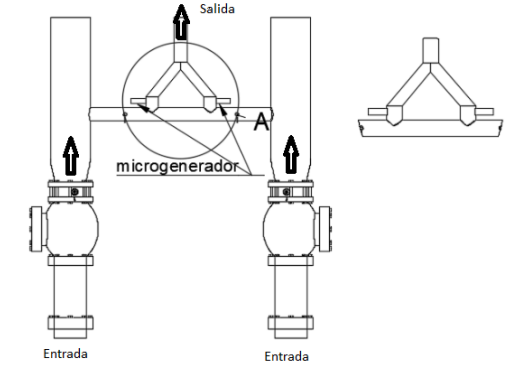
\includegraphics[width=\linewidth]{img/DisenoSub1.png}
        \end{subfigure}
        \begin{subfigure}{0.4\linewidth}
            \centering
            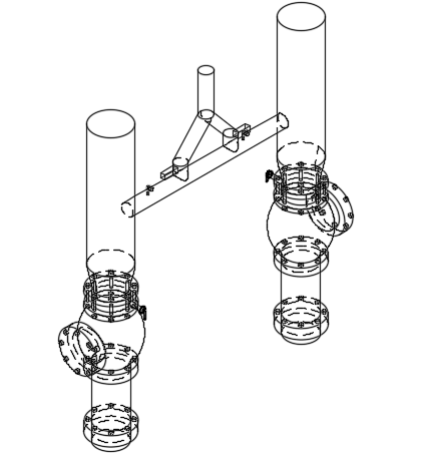
\includegraphics[width=\linewidth]{img/DisenoSun2.png}
        \end{subfigure}
        \begin{subfigure}{0.15\linewidth}
            \centering
            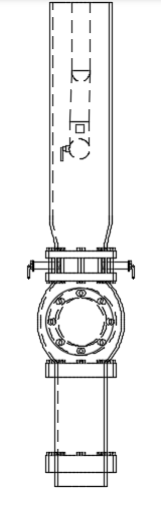
\includegraphics[width=\linewidth]{img/DisenoSub3.png}
        \end{subfigure} 

        \caption{Plano de diseño conceptual de la colocación de los microgeneradores}
    \end{figure}



    % === 10.
    \section{Recursos}
 
        \subsection{Recursos institucionales}
            \begin{itemize}
                \item Asesoría del tutor empresarial y técnicos del área de Mantenimiento Planta Común
                de la empresa Continental Tire Andina S.A.

                \item Asesoría del tutor académico del Instituto Universitario Tecnológico del Azuay
            \end{itemize}
  
        \subsection{Recursos materiales}
            \begin{itemize}
                \item Insumos de oficina.
            \end{itemize}
  
        \subsection{Recursos técnicos o tecnológicos}
            \begin{itemize}
                \item Computadora
                \item Celular
                \item Impresora.
                \item Software de Diseño Fusion 360.
                \item Internet.
            \end{itemize}
 
  
    % === 11.
    \section{Conclusiones y recomendaciones}

        \subsection{Conclusiones}
            \begin{itemize}
                \item La revisión de los fundamentos teóricos asociados a la generación de energía
                eléctrica mediante micro generadores hidroeléctricos proporcionó una base sólida
                para comprender todos los componentes del sistema y obtener una idea más precisa
                de la construcción deseada.
                
                \item Los sistemas de generación de energía eléctrica mediante micro generadores
                hidroeléctricos ofrecen beneficios significativos, como su sostenibilidad ambiental,
                bajo impacto ambiental y flexibilidad de ubicación. Sin embargo, también se
                destacan desafíos, como la dependencia de condiciones hidrológicas y los costos de
                implementación y mantenimiento.
                
                \item La viabilidad de implementar un sistema de generación de energía eléctrica
                utilizando micro generadores hidroeléctricos junto con una estación de carga para
                una empresa como Continental Tire Andina S.A. parece prometedora, ya que se
                anticipan beneficios en términos de sostenibilidad, eficiencia operativa y reducción
                de costos a largo plazo. Sin embargo, aún queda por analizar el costo de desarrollo
                del proyecto para determinar su viabilidad específica.
            \end{itemize}
  
        \subsection{Recomendaciones}
            \begin{itemize}
                \item Realizar un análisis detallado de los costos asociados con la implementación y
                operación del proyecto, incluyendo el costo de adquisición e instalación de los
                equipos, los costos de mantenimiento y reparación, y los posibles ahorros en
                términos de consumo de energía convencional.
                
                \item Calcular el retorno de inversión esperado del proyecto.
            \end{itemize}
     
    % === 12.
    \section{Referencias bibliográficas}
            \begin{itemize}
                \item Herrería Romero, B. D. (2022). Estudio comparativo de las tecnologías de
                almacenamiento de energía eléctrica (Bachelor's thesis).
                \url{http://repositorio.utn.edu.ec/bitstream/123456789/13272/2/04%20MEL%20174%20T
                RABAJO%20DE%20GRADO.pdf}
                
                \item Hernández Romero, A. (s/f). Baterías para Almacenamiento de Energía.
                Biblus.us.es. Recuperado el 25 de febrero de 2024, de 
                \url{https://biblus.us.es/bibing/proyectos/abreproy/70692/fichero/10+Baterias+para+Alma
                cenamiento+de+Energ%C3%ADa.pdf}
                
                \item Repsol. (2023). Energía hidráulica: qué es y qué ventajas tiene | Repsol. REPSOL.
                \url{https://www.repsol.com/es/energia-futuro/futuro-planeta/energia-hidraulica/index.csht
                ml}
                
                \item Sanz, M. (2021, julio 19). Microgeneradores de energía eléctrica. NextCity Labs.
                \url{https://nextcitylabs.com/global/es/microgeneradores-de-energia-electrica/
                }

                \item Ecuador, I. (2023, noviembre 13). Conoce los Tipos de Generadores Eléctricos y sus
                características. Inducom Ecuador. 
                \url{https://inducom-ec.com/conoce-los-tipos-de-generadores-} \\ \url{electricos-y-sus-caracteristi
                cas}
            \end{itemize}


   
    % === 13.
    \section{Contacto}

        \noindent \textit{\underline{Estudiante:}} Eduardo Mendieta. \\
        \textit{\underline{Celular:}} 098 881 6416 \\
        \textit{\underline{Correo electrónico:}} christian.mendieta.est@tecazuay.edu.ec \\\

        \noindent  \textit{\underline{Estudiante:}} Christian Sánchez. \\
        \textit{\underline{Celular:}}  096 795 6731.\\
        \textit{\underline{Correo electrónico:}} christiand.sanchez.est@tecazuay.edu.ec

    % === 14.
    \newpage
    \section{Anexos}
    
    \begin{figure}[htbp]
        \centering
        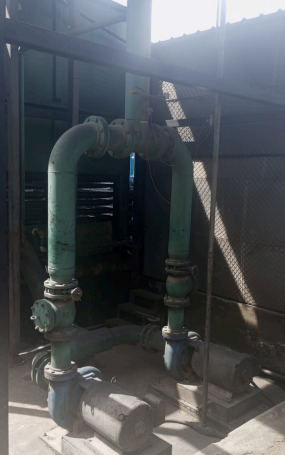
\includegraphics[width=0.3\linewidth]{img/Anexo1.png}
        \caption{Torre de enfriamiento}
    \end{figure}

    \begin{figure}[htbp]
        \centering
        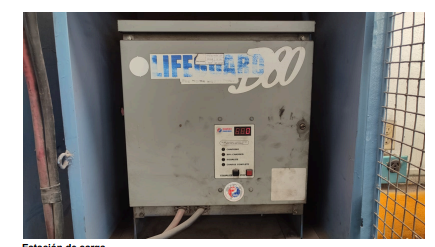
\includegraphics[width=0.5\linewidth]{img/Anexo2.png}
        \caption{Estación de carga}
    \end{figure}

    \begin{figure}[htbp]
        \centering
        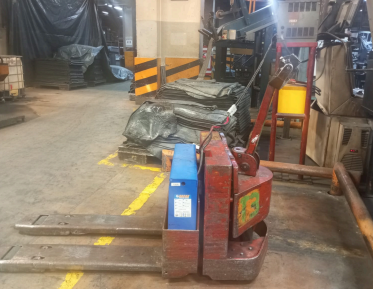
\includegraphics[width=0.4\linewidth]{img/Anexo3.png}
        \caption{Montacargas Prime Mover}
    \end{figure}

    \begin{figure}[htbp]
        \centering
        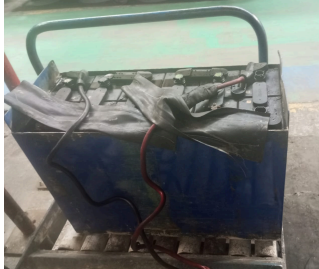
\includegraphics[width=0.4\linewidth]{img/Anexo4.png}
        \caption{Batería montacargas Prime Mover}
    \end{figure}

    \begin{figure}[htbp]
        \centering
        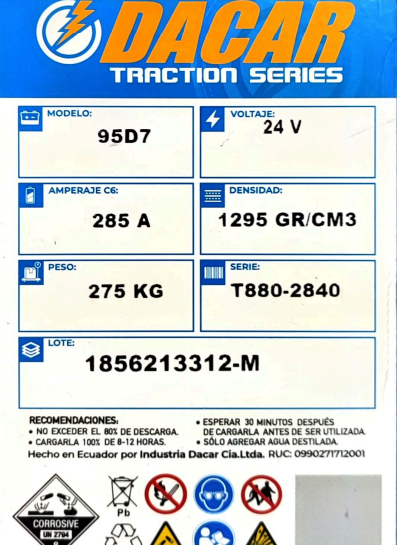
\includegraphics[width=0.3\linewidth]{img/Anexo5.png}
        \caption{Ficha técnica de la batería}
    \end{figure}

\end{document}
